\documentclass[border=5pt]{standalone}
\usepackage{tikz}
\usepackage{xcolor}
\usetikzlibrary{calc,shadows.blur}

% J10 - Green short ring
\begin{document}
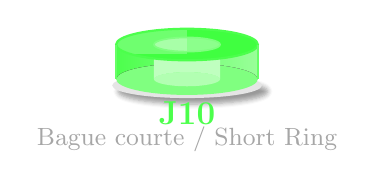
\begin{tikzpicture}

% Shadow
\fill[gray!20,blur shadow={shadow blur steps=5}] (0,-0.3) ellipse (0.95 and 0.16);

% Bottom annular face
\fill[green!50] (0,-0.22) ellipse (0.9 and 0.2);
\fill[green!30] (0,-0.22) ellipse (0.42 and 0.09);

% Outer side wall
\fill[left color=green!70, right color=green!40]
  (-0.9,-0.22) -- (-0.9,0.22)
  arc[start angle=180,end angle=0,x radius=0.9,y radius=0.2]
  -- (0.9,-0.22)
  arc[start angle=0,end angle=180,x radius=0.9,y radius=0.2];

% Inner hole wall
\fill[green!25]
  (-0.42,-0.22) -- (-0.42,0.22)
  arc[start angle=180,end angle=0,x radius=0.42,y radius=0.09]
  -- (0.42,-0.22)
  arc[start angle=0,end angle=180,x radius=0.42,y radius=0.09];

% Top annular face
\fill[green!75] (0,0.22) ellipse (0.9 and 0.2);
\fill[green!45] (0,0.22) ellipse (0.42 and 0.09);

% Highlight
\begin{scope}
  \clip (0,0.22) ellipse (0.9 and 0.2);
  \fill[white,opacity=0.25] (-0.95,0.1) rectangle (0.0,0.45);
\end{scope}

% Outlines
\draw[green!70, line width=0.8pt] (0,0.22) ellipse (0.9 and 0.2);
\draw[green!50, line width=0.6pt] (0,0.22) ellipse (0.42 and 0.09);
\draw[green!60, line width=0.7pt] (-0.9,-0.22) -- (-0.9,0.22);
\draw[green!60, line width=0.7pt] (0.9,-0.22) -- (0.9,0.22);

% Label
\node[font=\bfseries\large, text=green!70] at (0,-0.65) {J10};
\node[font=\small, text=gray!70] at (0,-0.98) {Bague courte / Short Ring};

\end{tikzpicture}
\end{document}
